\chapter{Všeobecné informácie o~aplikácii}

\section{Aspekty hľadania najrýchlejšej trasy (v OB)}\label{Aspekty_hladania}

Mapy pre~orientačný beh sú veľmi detailné, a~bežec má preto mnoho informácií na~to, aby~si mohol zvoliť ideálnu trasu. Za~predpokladu, že~bežec nerobí chyby a~beží presne podľa svojho zámeru, sú pre~výber najrýchlejšieho postupu dôležité dva druhy objektov: líniové (cesty, potoky, prieseky, vrstevnice, ...) a~plošné (lúky, kroviská, vodné objekty, močiare, ...). Tie určujú typ terénu nachádzajúci sa v~danej časti mapy a~tým pádom aj~veľkosť odporu, ktorý~je kladený rýchlosti behu pretekára. Táto veličina sa dá použiť ako hlavný parameter, ktorý~bude určovať preferencie výberu postupu.

Proces hľadania cesty sa skladá z~dvoch hlavných častí: 
\begin{itemize}
    \item \textbf{vytvorenie mapovej reprezentácie} - Na~začiatku je potrené na~základe mapového súboru vygenerovať mapovú reprezentáciu, na~ktorej bude možné cestu vyhľadávať. Mapovou reprezentáciou by mal byť objekt, ktorý~dobre vystihne topografiu mapy a~umožní hľadanie najideálnejšej trasy. V~našej aplikácii budú týmito objektmi \textit{orientované ohodnotené grafy}.  
    \item \textbf{aplikácia vyhľadávacieho algoritmu} - Mapová reprezentácia s vybraným užívateľským modelom sú predané vyhľadávaciemu algoritmu. Ten za~použitia interface-u mapovej reprezentácie a výpočtov užívateľského modelu vyhľadá v~mapovej reprezentácii najkratšiu cestu na zadanej trati. V~našom prípade najkratšia cesta znamená tá najrýchlejšia.
\end{itemize}

V~nasledujúcich podsekciách spomenieme koncepty, ktoré~budú v~procese hľadania najrýchlejších ciest vystupovať. Medzi jednotlivými konceptmi sú tvorené rôzne závislosti. Grafické znázornenie týchto závislostí je dostupné k nahliadnutiu na~konci sekcie v~Obrázku~\ref{obr01:konceptove_zavislosti}.   

\subsection{Mapy}\label{mapy}

Na začiatok je potrebné spomenúť koncept mapy. V~procese hľadania ciest bude na~viacerých miestach potrebné agregovať dáta z~užívateľom vybraného mapového súboru. Aby~sme nemuseli neustále čítať priamo zo~súboru, budeme si udržovať jeho obsah v~pamäti prívetivejším spôsobom. 

Touto formou bude práve \textit{mapa}. Mapa si bude udržovať všetky objekty definované v~mapovom súbore a~keď bude potrebné agregovať z~daného súboru nejakú informáciu (mapovú reprezentáciu, mapovú grafiku, ...), použije sa namiesto súboru zodpovedajúci mapový objekt.

Je vhodné zmieniť, že~koncept mapy je odlišný od konceptu \textit{mapovej reprezentácie}. Mapa, na~rozdiel od jej reprezentácie, neobsahuje žiadne zložité prepojenia medzi objektami ktoré~v~sebe drží. Jej vytvorenie by malo byť rýchle, s~lineárnou časovou zložitosťou v~závislosti od~veľkosti mapového súboru.

\subsection{Mapové reprezentácie}\label{mapove_reprezentacie}

Mapové reprezentácie sú jednou z~dôležitých zložiek procesu hľadania ciest. Sú to jednotky, na~ktorých sa vyhľadávanie uskutočňuje. Mapové objekty sú oproti \textit{mapám} zložitejšie objekty, ktoré~už v~sebe zahŕňajú plno závislostí a~prepojení. Ich generovanie môže zabrať oveľa viac času, ako generovanie mapových objektov. 

Ako už bolo spomenuté vyššie, v~aplikácii budú mapovými reprezentáciami \textit{orientované, ohodnotené grafy} (ďalej iba grafy). Napriek tomu, že~mapová reprezentácia a~graf budú v~aplikácii reprezentovať rovnaký objekt, ich významy sú odlišné:

\begin{itemize}
    \item \textbf{Mapová reprezentácia} hovorí o~tom, ako daný objekt pracuje interne. Popisuje jeho vlastnosti, mechanizmy a~spôsoby akými generuje výsledný \textit{graf}, v~ktorom sa následne hľadá cesta. Objekt, ktorý~je agregovaný z~mapy, je v~prvom rade mapovou reprezentáciou a~až v~druhom rade grafom.
    
    Príkladom myšlienky, ktorú môže mapová reprezentácia vyjadrovať je \uv{samo-zahusťujúci} sa graf. Takáto mapová reprezentácia počas behu algoritmu zahusťuje predom pripravený graf o~ďalšie vrcholy na~miestach, v~ktorých sa prehľadávanie aktuálne uskutočňuje. Redukuje sa tým veľkosť predom vygenerovaného grafu a~zvyšuje jeho presnosť na~miestach, kde je to potrebné.   
    \item\textbf{Graf} na~druhej strane hovorí o~vlastnostiach objektu, ktoré~sú viditeľné navonok. Bude informovať o~\uv{grafových} službách objektu, ktoré~dokáže poskytnúť. Tieto služby môžu byť obmedzené práve vnútornou štruktúrou ktorá je definovaná \textit{mapovou reprezentáciou}. Graf sa berie ako druhotný produkt spracovania mapy.   

    Príkladom vlastnosti, ktorú môže graf prezentovať vonkajšiemu svetu, je možnosť poskytnutia kompletne vygenerovaného grafu, pri~ktorom sa vonkajší užívateľ nemusí obávať, že~by sa počas práce s~ním graf nejakým spôsobom modifikoval. Túto vlastnosť napríklad nevie zaručiť graf ktorý~zodpovedá vyššie zmienenej mapovej reprezentácii, ktorá stav~grafu počas práce neustále modifikuje, zahusťuje ho.
\end{itemize}

Pojmy \textit{mapová reprezentácia} a~\textit{graf} reprezentujú dve odlišné myšlienky a~v~texte budú na~ich základe aj~využívané. Je však potrebné mať na~pamäti, že~v~aplikácii sú tieto pojmy jednou a~tou istou dátovou štruktúrou. Z~hľadiska vytvárania a~používania sa teda mapová reprezentácia a~graf stávajú zameniteľnými.

\subsection{Užívateľské modely}\label{uzivatelske_modely}

Je potrebné si uvedomiť, že~rôzni bežci majú rôzne schopnosti a~preto aj~ich preferencie na~výber trasy nemusia byť rovnaké. Niekto sa dokáže rýchlejšie predierať cez husté pasáže, inému ide rýchlejšie beh cez močiar a~ďalšiemu vyhovujú dlhšie postupy po~cestách. 

Preto by bolo vhodné, aby~užívateľ aplikácie mal možnosť aplikovať svoje preferencie do~procesu vyhľadávania. K~tomuto účelu boli vytvorené tzv. \uv{užívateľské modely}. Užívateľ si pomocou nich môže vytvoriť vlastný \uv{profil}, na~základe ktorého bude vyhľadávanie cesty prispôsobené.

Užívateľské modely vďaka svojej informovanosti nadobúdajú zodpovednosť za~výpočty hodnôt, ktoré~sú závislé na~preferenciách užívateľa. Stávajú sa teda dôležitou zložkou procesu vyhľadávania ciest, nakoľko vyhľadávacie algoritmy sú závislé do~nimi vykonávaných výpočtov.

\subsection{Výškové dáta}\label{vyskove_data}

Jedným z~dôležitých a~neopomenuteľných faktorov~voľby najrýchlejšieho postupu je prevýšenie, ktoré~je potrebné pri~jeho prevedení zdolať. Mnoho typov~máp popisuje reliéf krajiny pomocou takzvaných \textit{vrstevníc}. Vrstevnica je krivka na~mape, ktorá spája body rovnakej nadmorskej výšky. Pre~človeka je vrstevnicová abstrakcia výšky terénu veľmi ľahko pochopiteľná a~spracovateľná.

Pre strojové spracovanie mapy však vrstevnice predstavujú veľmi neprirodzený spôsob reprezentácie nadmorskej výšky. Vypracovanie reliéfneho obrazu za~pomoci vrstevníc samotných je veľmi ťažká úloha. V~niektorých prípadoch (mapy pre~OB napríklad) dokonca jednotlivé vrstevnice nie sú v~mapovom súbore reprezentované jedným objektom, nakoľko sú kvôli dobrej čitateľnosti máp na~viacerých miestach prerušované.
%TODO: mozno najst nejaku tu pracu co sa tym zaoberala, zistit od risa, odkazat na~nu

Z~vyššie uvedených dôvodov je v~aplikácii zahrnutý systém, ktorý~sprostredkováva užívateľom možnosť stiahnutia a~spravovania digitálnych výškových dát, ktoré~následne môžu byť použité ako pomocný zdroj v~procese tvorby mapových reprezentácií. Pre~konštrukciu mapových reprezentácií pre~niektoré mapové formáty bude nutná prítomnosť zodpovedajúcich výškových dát a~pri ich absencii jednoducho nebude možné mapové reprezentácie vytvoriť.

Výškové dáta môžu byť sťahované z~viacerých zdrojov. Každý zdroj môže definovať viacero dátových distribúcií, ktoré~dokáže ponúknuť. Tieto distribúcie sa väčšinou líšia kvalitou a~dostupnosťou sprostredkovaných dát (v~niektorých prípadoch je k~stiahnutiu výškových dát potrebná užívateľova autorizácia).

\subsection{Atribútové template-y}\label{templatey}

Ďalšia vec, nad ktorou je potrebné sa zamyslieť je, akým spôsobom sa bude v~grafoch mapových reprezentácií uchovávať informácia o~mapových vlastnostiach a~atribútoch, ktoré~konkrétne vrcholy a~hrany grafu reprezentujú. Zároveň je potrebné aby~dotyčné vlastnosti dokázal príslušný užívateľský model spracovať a~dopočítať z~nich hodnoty, potrebné pre~beh vyhľadávacích algoritmov. Používané atribúty, ktoré~agregujeme z~máp do~mapových reprezentácií preto musia byť jednotné v~celom procese hľadania cesty, od vytvárania mapovej reprezentácie, po~spustenie vyhľadávacieho algoritmu.

V~aplikácii nám definíciu a~jednotnosť atribútov budú zabezpečovať tzv. \textit{template}-y. Každý template bude definovať jedinečnú sadu vrcholových a~hranových atribútov. Príkladom pre~takúto kolekciu pre~potreby OB môže byť napríklad:
\begin{itemize}
    \item vrcholové atribúty - pozícia, výška, indikátory reprezentovaných terénnych objektov (či~sa daný vrchol nachádza na~ceste, v~húštine, na~lúke, v~dobre priebežnom lese,...),
    \item hranové atribúty - či~daná hrana reprezentuje úsek nejakej cesty, hranu nejakého objektu (lúky, húštiny, močiaru,...), sklon terénu
\end{itemize}

Na template-och ako takých bude teda závisieť: 
\begin{itemize}
    \item \textbf{výber užívateľských modelov} - model musí vedieť spracovať atribúty definované daným template-om a~vrátiť od neho požadované výsledky.
    \item \textbf{formát vybraného mapového súboru} - musí existovať konvertor mapy špecifického formátu na~zodpovedajúcu mapovú reprezentáciu, v~ktorej vrcholoch a~hranách sú obsiahnuté atribúty definované daným template-om. Túto závislosť môžeme brať aj~opačným smerom - pre~vybraný mapový formát môžeme zvoliť len použiteľný template.
\end{itemize}

\subsection{Vyhľadávacie algoritmy}\label{vyhladavacie_algoritmy}

Nakoniec nemôžeme opomenúť koncept samotných vyhľadávacích algoritmov, poslednú neodmysliteľnú súčasť procesu hľadania ciest. Vyhľadávací algoritmus, podobne ako \textit{mapová reprezentácia}, reprezentuje koncept vnútorného mechanizmu ktorým je najkratšia cesta v~grafe hľadaná. Príkladom takéhoto algoritmu môže byť napríklad algoritmus \textit{A*}. 

Vstupom do~každého algoritmu sú:
\begin{itemize}
    \item \textbf{graf}, na~ktorom je hľadanie najkratšej cesty vykonané a~
    \item \textbf{užívateľský model}, ktorý~algoritmus nutne potrebuje k~výpočtom váh grafových hrán a~iných hodnôt potrebných k~jeho správnemu chodu.  
\end{itemize}

Každý algoritmus následne ponúka množinu jeho implementácií. Každá implementácia definuje množinu vlastností, ktoré~vložený graf a~užívateľský model musia spĺňať. Napríklad implementácie A* algoritmu budú požadovať, aby~užívateľský model bol schopný popri výpočte váh pre~grafové hrany, dodať ešte aj~výpočet heuristiky využívanej týmto algoritmom.

Stav používaného grafu sa môže počas behu algoritmu meniť. Teda je potrebné ho vždy na~konci vyhľadávania opäť vrátiť do~pôvodného stavu a~zaručiť, že~graf je v~jednu chvíľu súčasťou len jedného vyhľadávacieho procesu.

Vyhľadávanie samotné je sprostredkované dvomi spôsobmi. Buď sa požiada algoritmus priamo o~nájdenie cesty na~danej trati alebo~sa využije takzvaný \textit{executor} algoritmu. 

Executor nám sprostredkuje vybraný algoritmus, ktorý~bude pracovať s~dodanou mapovou reprezentáciou a~užívateľským modelom. Executor si pri~inicializácii pre~seba uzamkne dodanú mapovú reprezentáciu a~až do~jeho uvolnenia ju neodblokuje. Do~tejto doby môže prijímať rôzne vstupné trate a~vracať pre~nenájdené cesty. Hlavná výhoda executor-ov je práve ich schopnosť uzamknutia mapovej reprezentácie na~dlhšiu dobu. Vďaka tomu ju dokážu využívať pre~viacero separátnych vyhľadávaní, bez potreby jej neustáleho uvádzania do~konzistentného stavu.  

\begin{figure}[h]\centering
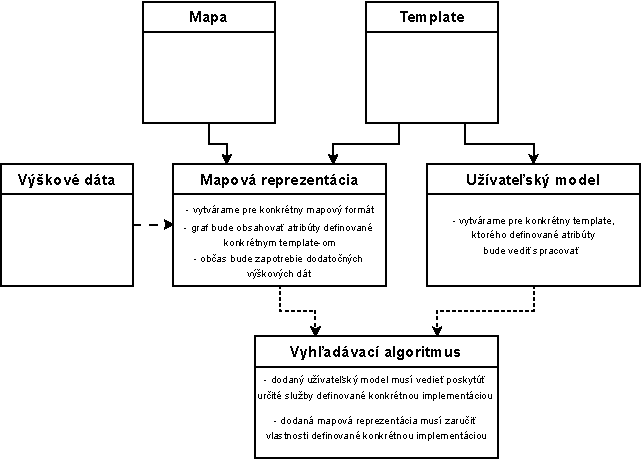
\includegraphics[]{img/konceptove_zavislosti}
\caption{Diagram závislostí jednotlivých konceptov} 
\label{obr01:konceptove_zavislosti}
\end{figure}

\pagebreak

\section{Zvolené implementačné prostriedky}

\subsection{Použitý programovací jazyk}

Pre implementáciu aplikácie bol vybraný jazyk C\#. Jazyk bol vybraný pre~jeho jednoduchosť a~bezpečnosť použitia. Alternatívnou volbou by mohol byť jazyk Java, ktorý~má blízko práve k~jazyku C\#. Voľba však padla na~C\# pre~široký výber možných framework-ov pre~implementáciu GUI. 

Ďalšími možnosťami by mohol byť typicky vysoko-úrovňový jazyk Python alebo~nízko úrovňový jazyk C++. Nakoľko v~aplikácii bude prebiehať mnoho výpočtov, Python by nebol vhodnou voľbou pre~nedostatočnú rýchlosť ním vytvoreného strojového kódu. Na~druhú stranu, C++ by bol dobrým kandidátom z~hľadiska výpočtovej sily. V~tomto prípade však narážame na~programátorskú neprívetivosť tohto jazyka. Pri~takomto väčšom projekte sme považovali za~potrebné mať istotu, že~nás použitý jazyk v~programovaní podrží. 

Vhodnou úpravou implementácie by bolo implementovať výpočtovo náročné procesy v~jazyku typu C++ a~následne túto implementáciu volať externe z~C\# jadra.     

\subsection{Užívateľské rozhranie}

Pre implementáciu užívateľského rozhrania sme sa rozhodli pre~\textit{Avalonia UI} framework. Užívateľské rozhranie je veľmi jednoduché. Bolo vytvorené tak, aby~zabezpečilo všetku funkcionalitu.

V~C\# existuje viacero možných knižníc, z~ktorých bolo možné si vybrať:
\begin{itemize}
    \item GUI knižnice, ktoré~sú súčasťou samotného .NET framework-u:
    \begin{itemize}
        \item \textbf{Windows Forms} je klasická GUI knižnica. Je jednoducho použiteľná a~vďaka jej dlhoročnej podpore aj~robustná a~spoľahlivá. Jej vek je však aj~jej nevýhodou, nakoľko vzhľad aplikácií vytvorených za~pomoci Windows Forms pôsobí pomerne zastaralo. Ďalšou nevýhodou je rastrová povaha jeho renderovcieho engine-u. Táto vlastnosť sa nehodí pre~aplikáciu, ktorej jedným z~hlavných účelov je vykresľovanie mapových, vektorových objektov.     
        \item \textbf{Windows Presentation Foundation (WPF)} je modernejší nástupca Windows Forms. Aplikácie tvorené touto knižnicou majú modernejší vzhľad a~sú generované renderovacím enginom založeným na~vektorovej grafike. K~programovaniu sa tu využíva popri C\# aj~XAML, v~ktorom sa definuje layout užívateľského rozhrania. Avšak spoločne s~Windows Forms je ich nevýhodou platformová závislosť na~operačnom systéme Windows.
        \item \textbf{.NET MAUI} je nástupcom \textit{Xamarin.Forms}. Je to open-source-ový cross-platformný framework s~množinou UI nástrojových balíčkov pre~jednotlivé platformy. Podobne ako vo~WPF sa pre~vytváranie UI využíva kombinácia C\# a~XAML. 
    \end{itemize}
    \item Alternatívou k~vstavaným .NET GUI knižniciam je práve nezávislá, open-source knižnica \textbf{Avalonia UI}. Čo sa vlastností je veľmi dobre porovnateľná s~\textit{.NET MAUI}. Hlavný rozdiel medzi týmito dvomi knižnicami je v~spôsobe, akým vykresľujú užívateľské rozhranie. Avalonia zapája kresliaci engine poháňaný knižnicou pre~2D grafiku \textit{Skia}. Na~druhú stranu MAUI využíva natívne nástrojové balíčky pre~každú platformu zvlášť. Ďalším rozdielom je, že~Avalonia, na~rozdiel od MAUI, podporuje aj~niektoré distribúcie Linuxových systémov.
\end{itemize}

Rozhodnutie nakoniec padlo na~využitie framework-u Avalonia UI. Nakoľko je veľmi podobný natívnemu .NET MAUI, rozhodla podpora pre~Linuxové systémy a~aj kvalitne spravená dokumentácia, z~ktorej sa dalo ľahko  vyčítať, ako sa s~knižnicou má pracovať. 

Informované rozhodnutie pre~výber GUI knižnice bolo učinené na~základe zdrojov \cite{WpfGuide,WhatIsMAUI,AvaloniaMauiComparison}. Zároveň väčšinu informácií, ktoré~sme o~Avalonia UI počas tvorby programu čerpali, pochádzali z~jej dokumentácie \cite{AvaloniaDokumentacia}.

\subsection{Architektúra Model-View-ViewModel (MVVM)}\label{ArchitekturaMVVM}

Jeden z~ďalších dôležitých aspektov, ktorý~hral úlohu vo~výbere knižnice pre~užívateľské rozhranie, bola podpora \textit{MVVM} návrhového vzoru. Dokumentácia Avalonia UI v preklade popisuje architektúru MVVM následovne: \uv{Model-View-View Model (MVVM) návrhový vzor je bežný spôsob štruktúrovania aplikácie užívateľského rozhrania. Používa systém viazania dát, ktorý~pomáha presúvať dáta medzi jeho časťami view-om a~view model-om. To znamená, že~dosahuje oddelenie aplikačnej logiky (view model) od~zobrazenia užívateľského rozhrania (view). Oddelenie medzi aplikačnou logikou a~obchodnými službami (model) sa bežne dosahuje pomocou systému Dependency Injection (DI).}\cite{MVVMDefByAvalonia}.

% The Model-View-View Model (MVVM) pattern is a~common way of structuring a~UI application. It uses a~data binding system that helps move data between its view and view model parts. This means it achieves separation of application logic (view model) from the display of the UI (view). Separation between the application logic and the business services (model) is commonly achieved by a~Dependency Injection (DI) system. 

MVVM architektúra je vhodná pre~našu aplikáciu, nakoľko pre~jej rozsah a~komplexnosť by klasická \textit{event-driven code-behind} architektúra nemusela postačovať. Týmto spôsobom zaručíme lepšiu separáciu a~dostatočnú vnútornú nezávislosť kódu.    

V~našej aplikácii bude tento návrhový vzor uplatnený s~jemnou obmenou. Vrstva View model, ktorá v~pôvodnom návrhovom vzore zastávala úlohu logiky aplikácie, bude rozdelená na~dve časti: View model a~novovzniknutý \textit{Model view}. Viac informácií o~tejto úprave je možné nájsť v~Sekcii~\ref{MVVMNavrhovyVzor}. 

\subsection{Reaktívne programovanie}

Ďalším dôležitým aspektom aplikácie je Avaloniou a~architektúrou MVVM iniciované využitie \textit{reaktívneho programovania.} Avalonia pre~aplikáciu tejto paradigmy využíva framework \textbf{Reactive UI}. 

Tento framework v preklade definuje reaktívne programovanie ako \uv{Reaktívne programovanie je programovanie s~asynchrónnymi dátovými tokmi.} a~dodáva \uv{Event bus-y alebo~typické udalosti kliknutia sú v~podstate asynchrónny tok udalostí, ktorý~je možné sledovať a~vykonávať na~ňom vedľajšie úkony. Reaktívne programovanie je táto myšlienka na~steroidoch. Je možné vytvárať dátové toky z~čohokoľvek, nielen z~udalostí kliknutia a~pohybu myši. Tieto toky sú lacné a~všadeprítomné, a~čokoľvek môže byť tokom: premenné, vstupy od používateľa, vlastnosti, cache, dátové štruktúry, atď.}\cite{ReactiveProgrammingByReactiveUI}.

% Reactive programming is programming with asynchronous data streams.
% Event buses or your typical click events are really an asynchronous event stream, on which you can observe and do~some side effects. Reactive programming is that idea on steroids. You are able to create data streams of anything, not just from click and hover events. Streams are cheap and ubiquitous and anything can be a~stream: variables, user inputs, properties, caches, data structures, etc.

V~aplikácii sa bude tento framework využívať prevažne vo~vrstvách View a~View model, medzi ktorými prebieha väčšina reaktívnej komunikácie. 